The ideal $K_{S}$ sample to estimate the systematic uncertainty in track and vertex reconstruction should have the same kinematic distributions as the $Z'$ MC sample. Obviously, the two samples have different distributions. Figure~\ref{fig:Ks_zp_comparison} shows comparisons of the vertex/kenematic distributions. The reconstructed $K_{S}$ and $Z'$ vertices are required to match to a $K_{S}$ and $Z'$ vertex produced at truth level with spatial displacement no larger than $0.7$ mm. All distributions are normalized to unity. It is fortuitous that their distribution cover the $r$ region of interest, and the two samples have similar $z$ distribution.


\begin{figure}[!htb]
    \centering
    \subfloat[]{\label{subfig:Ks_zp_r}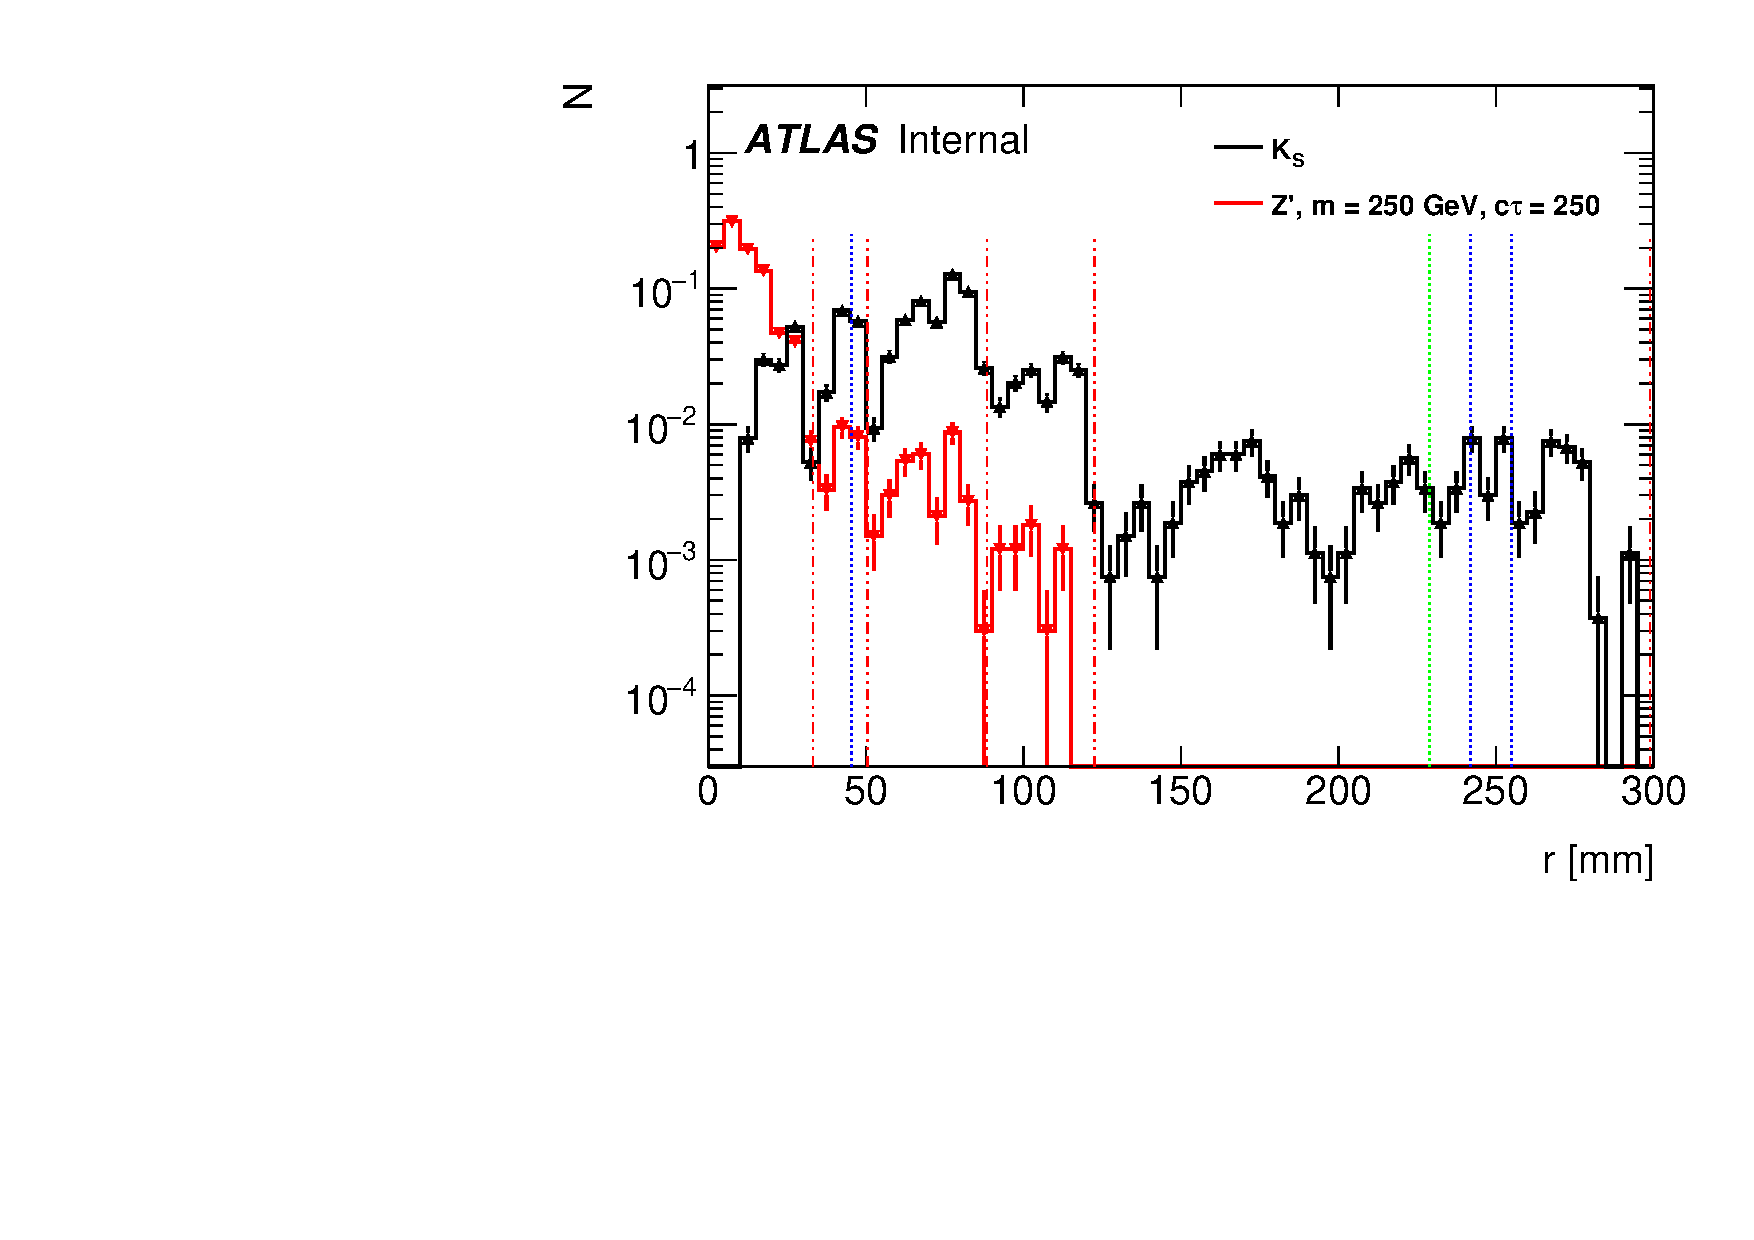
\includegraphics[width=0.40\textwidth]{figures/m_syst_zp_Ks_r.pdf}}
    \subfloat[]{\label{subfig:Ks_zp_z}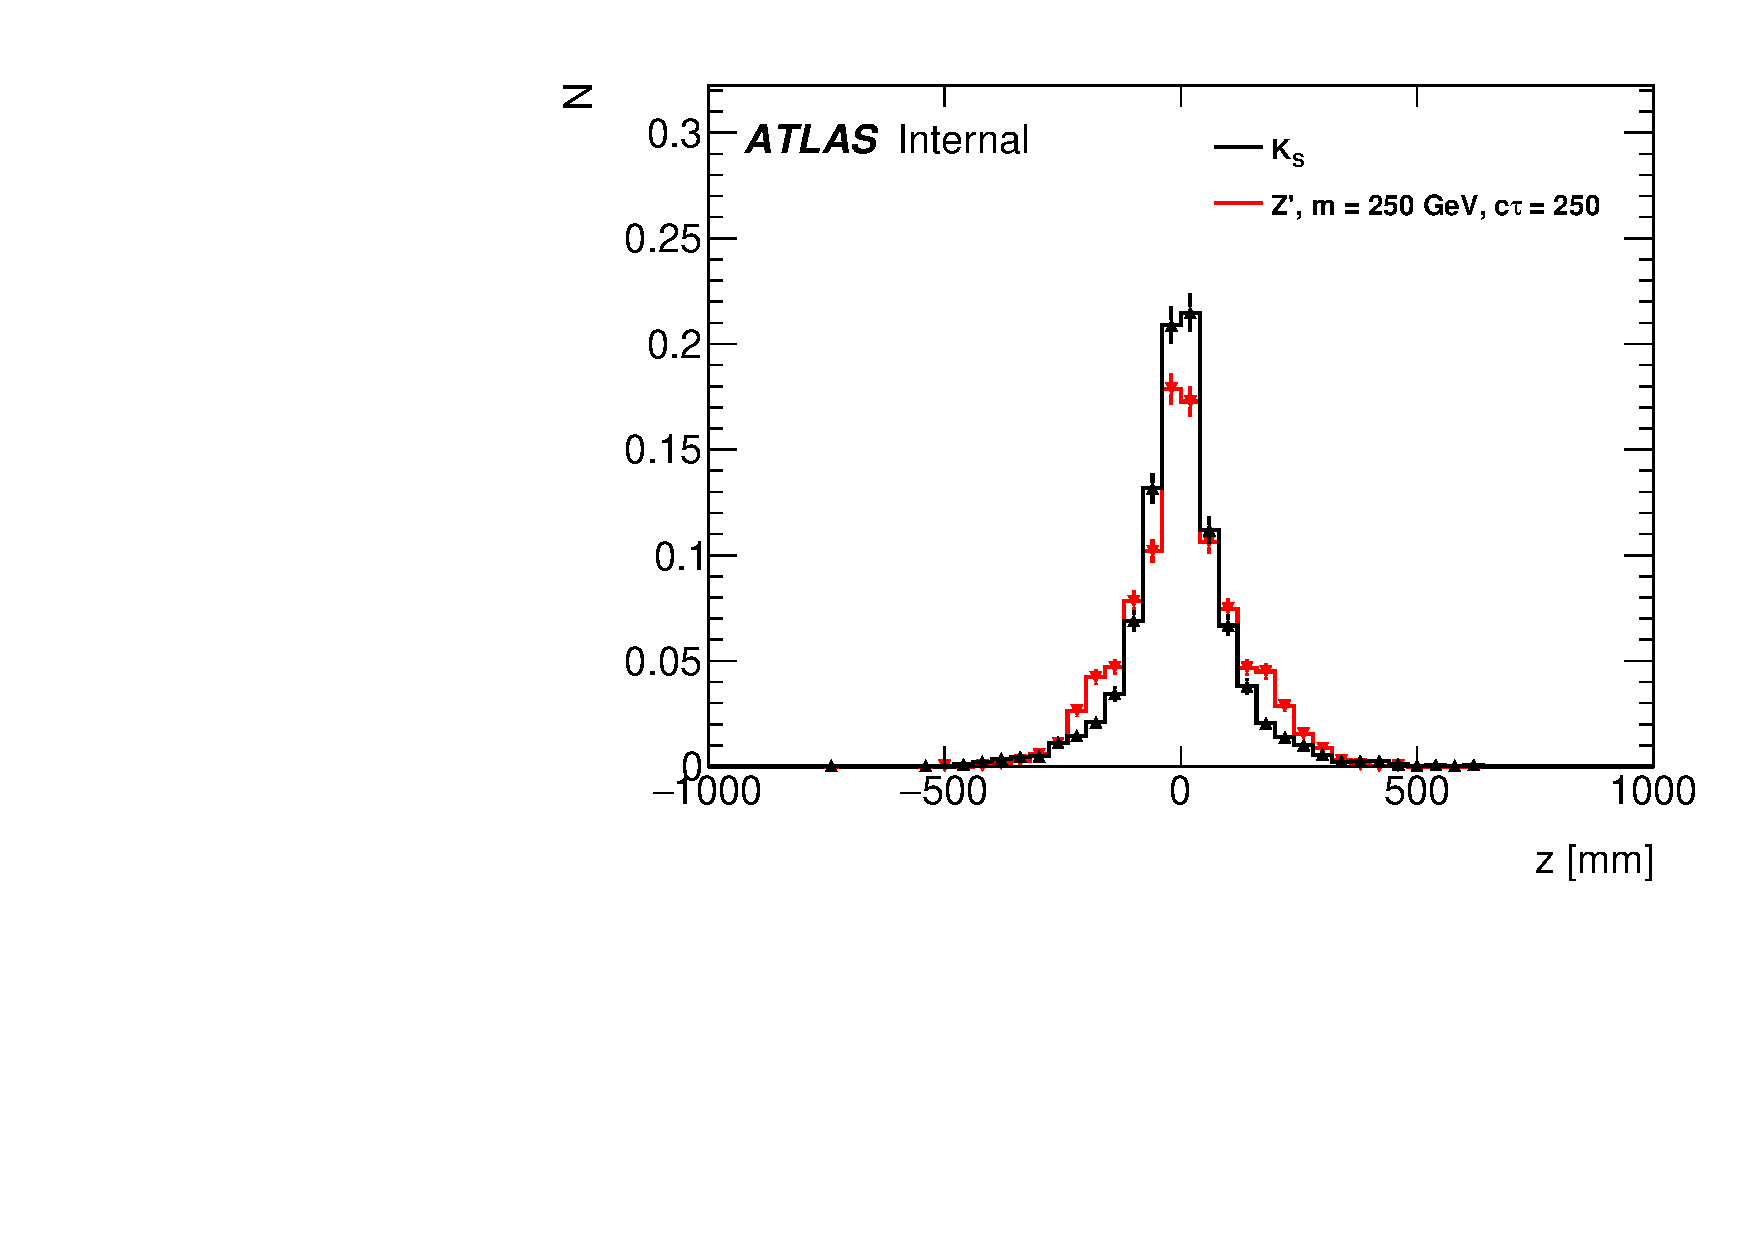
\includegraphics[width=0.40\textwidth]{figures/m_syst_zp_Ks_z.pdf}} \\
    \subfloat[]{\label{subfig:Ks_zp_eta}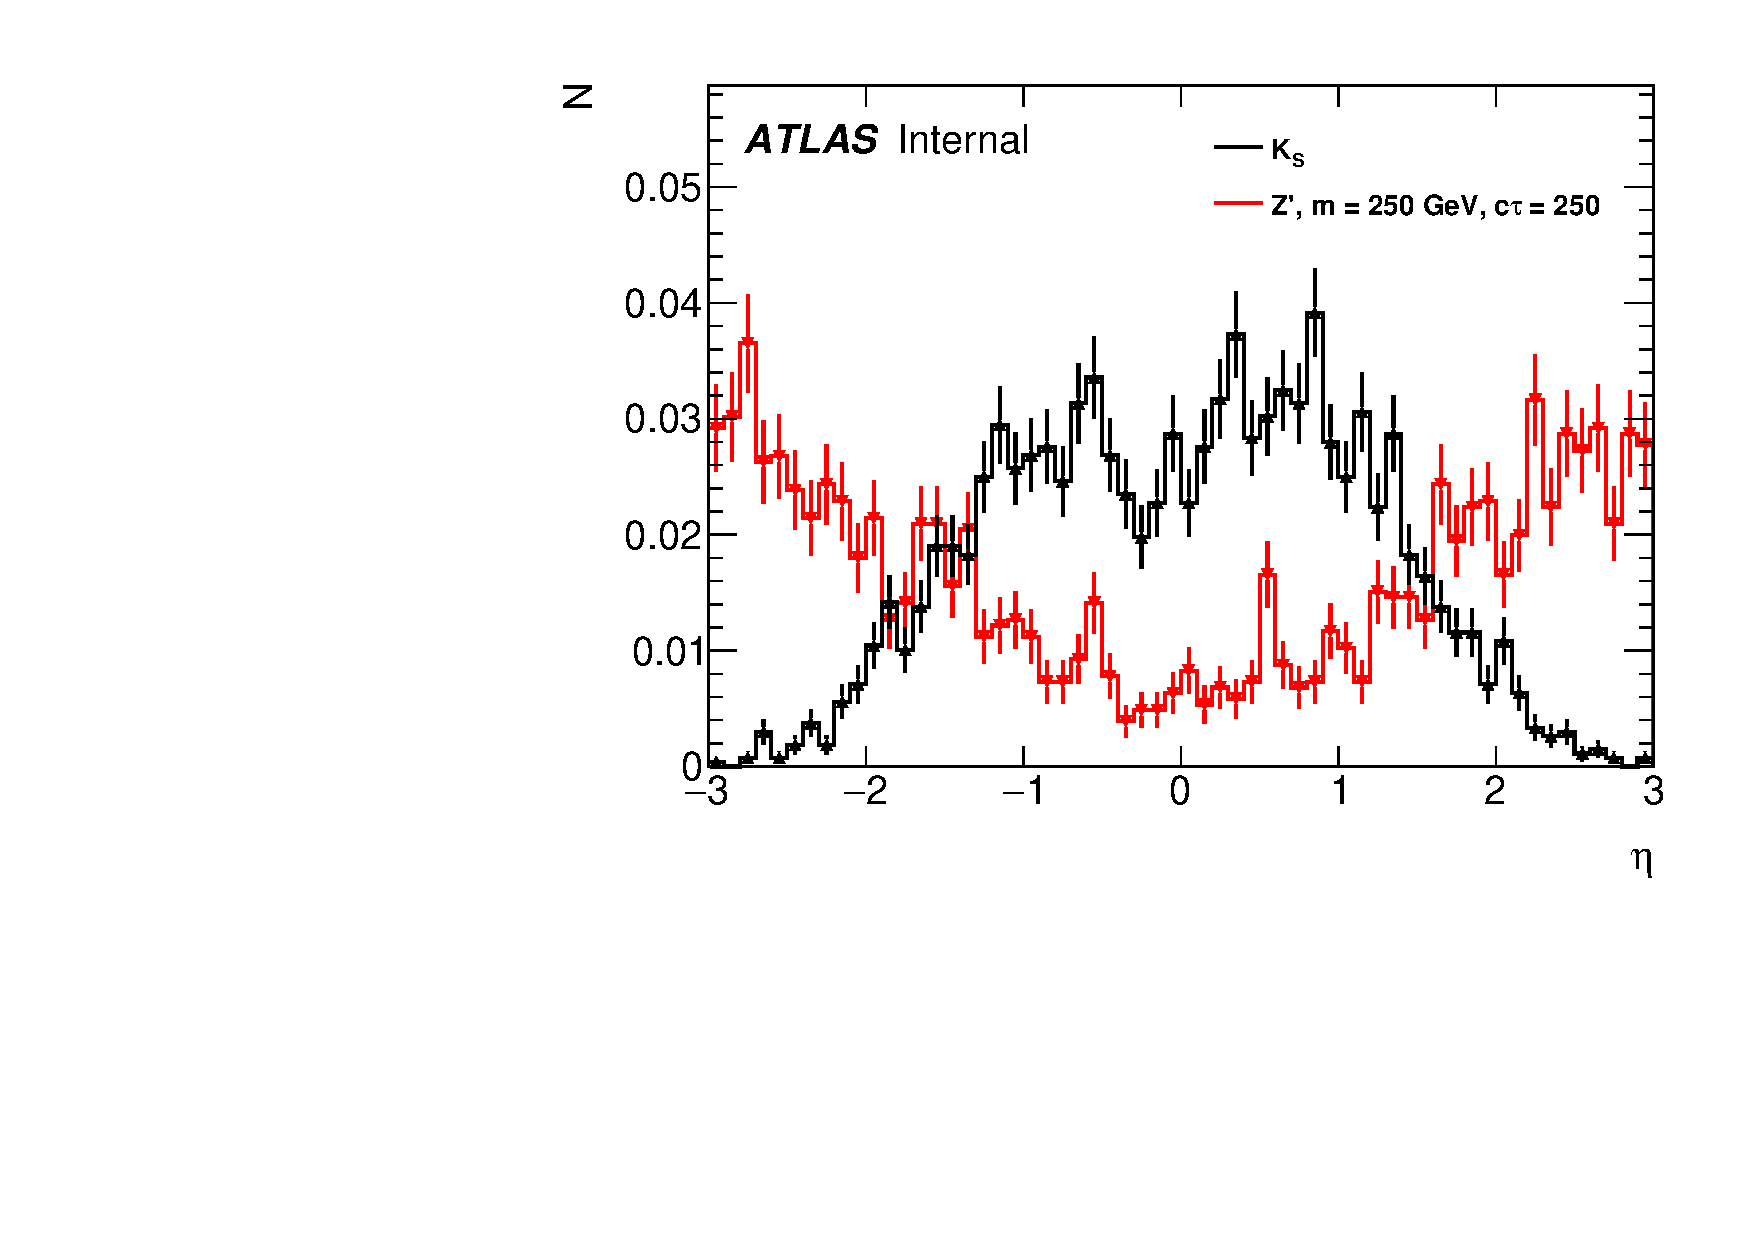
\includegraphics[width=0.40\textwidth]{figures/m_syst_zp_Ks_eta.pdf}} 
    \subfloat[]{\label{subfig:Ks_zp_pt}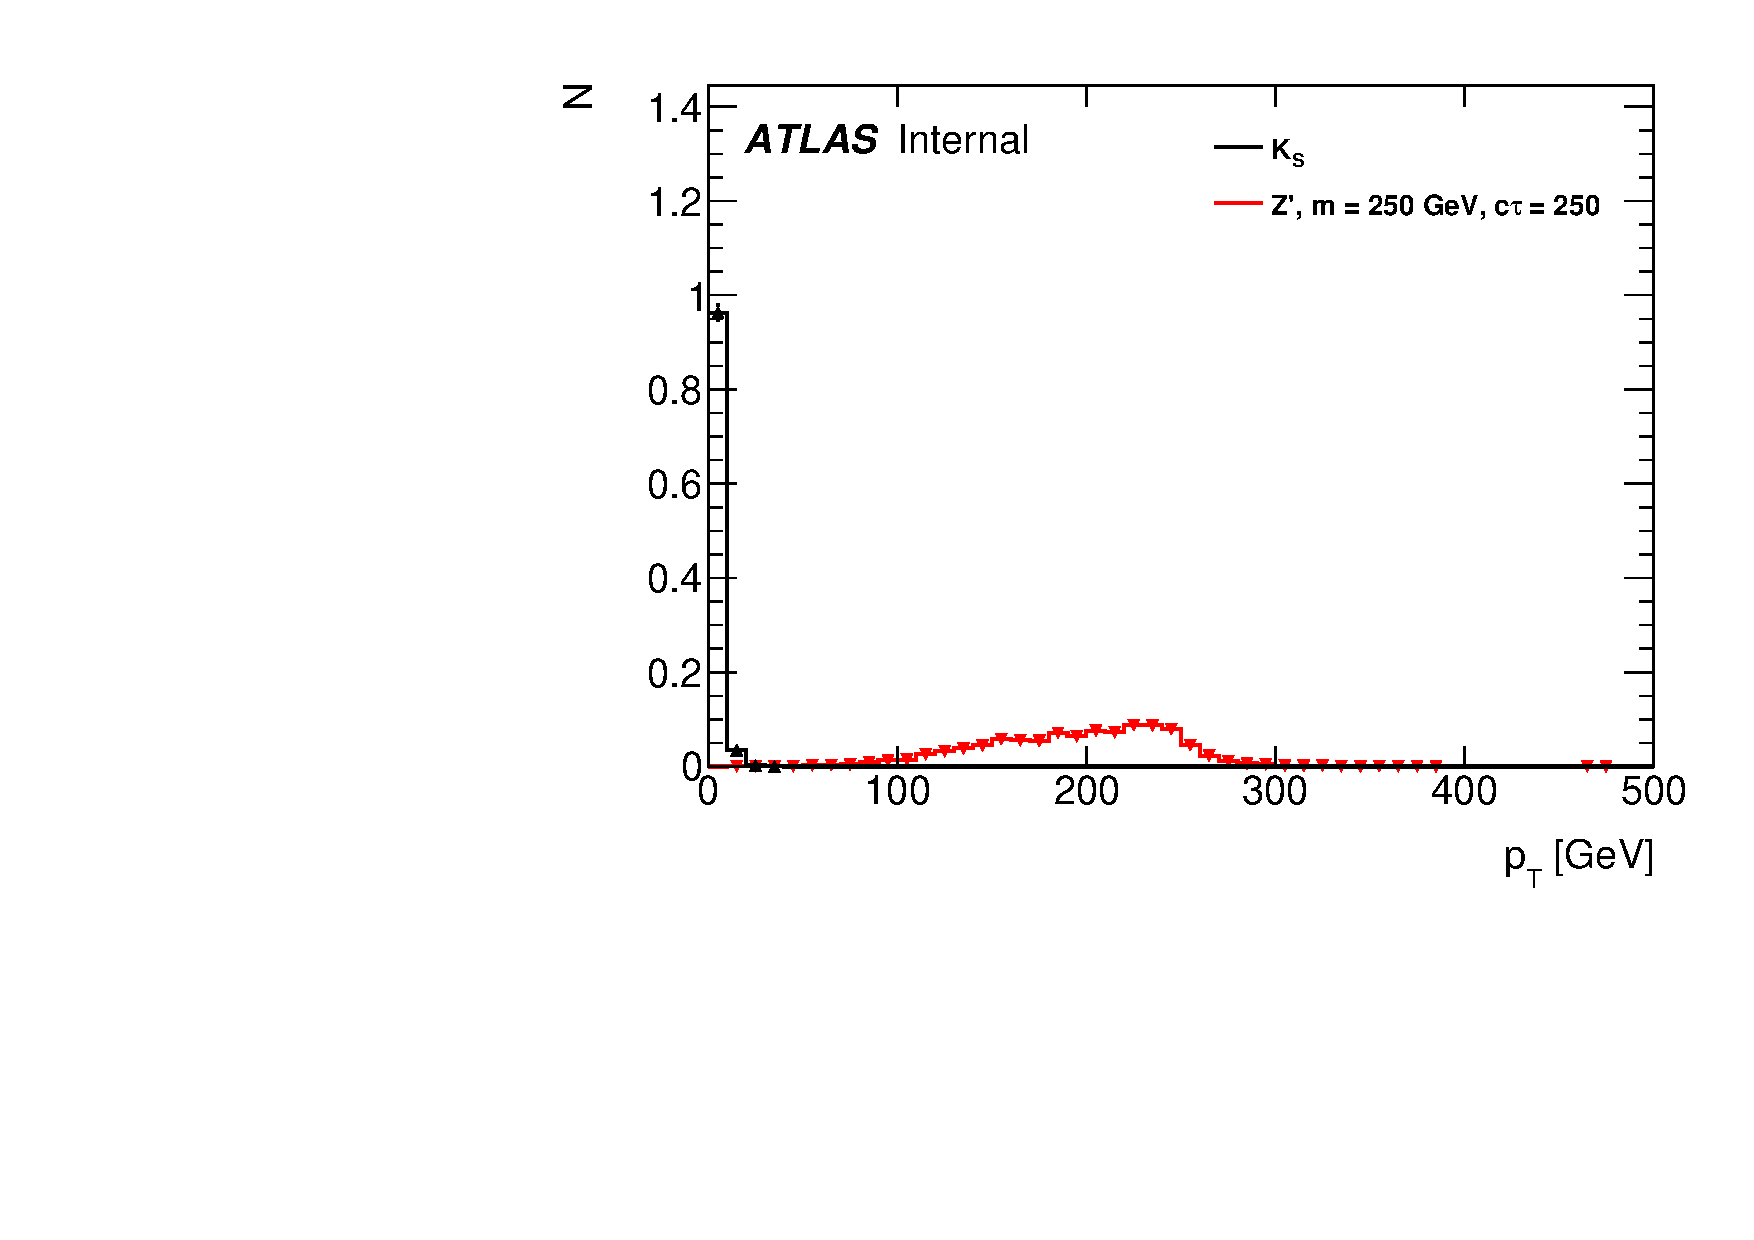
\includegraphics[width=0.40\textwidth]{figures/m_syst_zp_Ks_pt.pdf}} \\
    %\subfloat[]{\label{subfig:Ks_zp_z}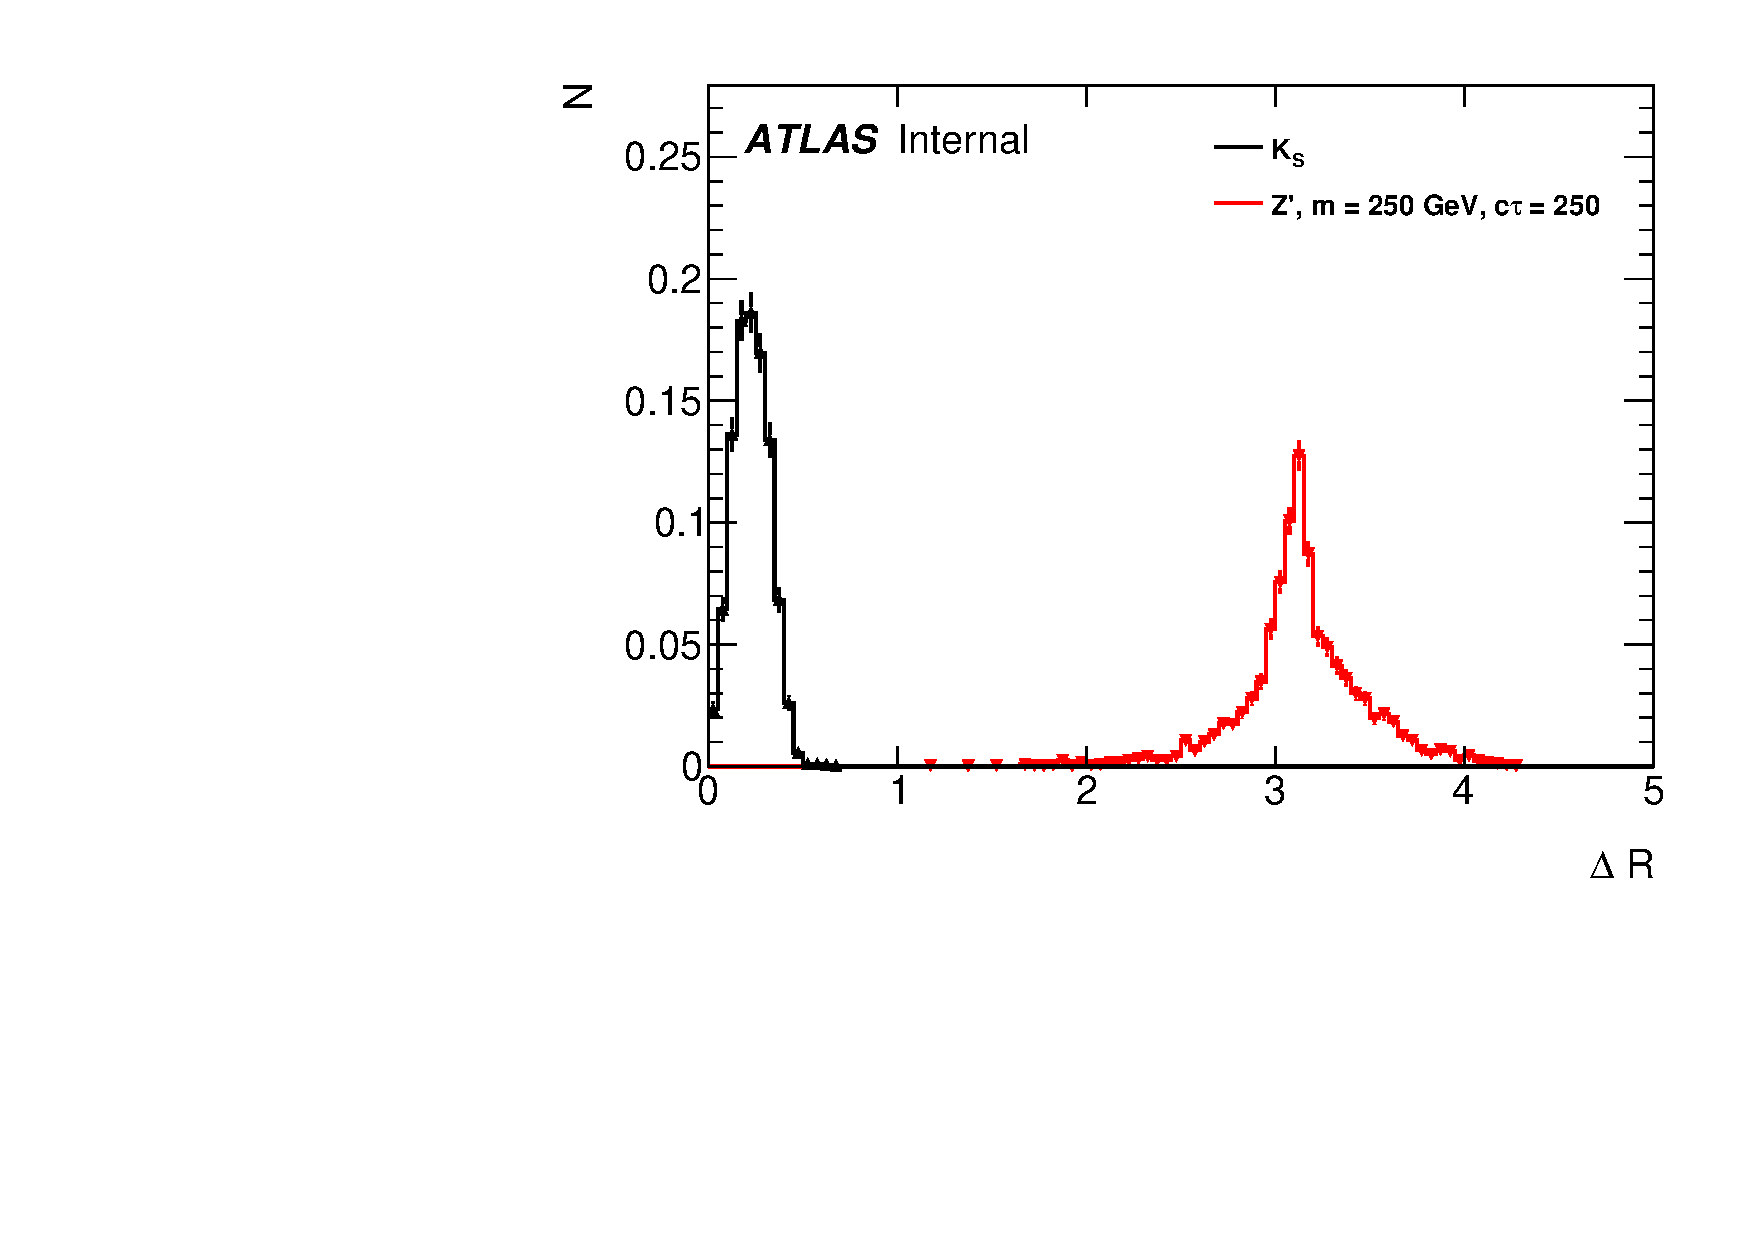
\includegraphics[width=0.40\textwidth]{figures/m_syst_zp_Ks_DeltaR.pdf}}
    \caption{Distribution of transverse (a), longitudinal vertex position (b), $\eta$ (c), $p_{T}$ (d), and the opening angle between decay particles of $K_{S}$ and $Z'$ vertices (e) found in the background and the signal MC sample described in Section~\ref{sec:vertexing_systematics_Ks_zp_comparison}. Distributions are normalized to unity. Systematic uncertainties are shown.}
    \label{fig:Ks_zp_comparison}
\end{figure}

